\documentclass[11pt,a4paper]{article}
\usepackage[T1]{fontenc}
\usepackage[utf8]{inputenc}
\usepackage{lmodern}
\usepackage[margin=23mm,headheight=15pt]{geometry}
\usepackage{amsmath,amssymb,bm}
\usepackage{booktabs,tabularx,array}
\usepackage{enumitem,microtype}
\usepackage{xcolor,tikz}
\usetikzlibrary{arrows.meta,positioning,calc,fit}
\usepackage{listings}
\usepackage{fancyhdr}
\usepackage{hyperref}
\definecolor{navy}{HTML}{193B54}
\definecolor{teal}{HTML}{087E8B}
\definecolor{pale}{HTML}{EAF4F5}
\definecolor{amber}{HTML}{B36B19}
\definecolor{missing}{HTML}{E0E4E8}
\hypersetup{colorlinks=true,linkcolor=navy,urlcolor=teal,citecolor=teal,
  pdftitle={AGFL-inm: Tensor representations for EEG channel-loss robustness},
  pdfauthor={Repository orientation document},pdfsubject={Mathematical concept and implementation review}}
\pagestyle{fancy}
\fancyhf{}
\fancyhead[L]{\small\textcolor{navy}{AGFL-inm\quad Concept and implementation}}
\fancyhead[R]{\small 1 October 2026}
\fancyfoot[R]{\thepage}
\renewcommand{\headrulewidth}{0.3pt}
\setlength{\parindent}{0pt}
\setlength{\parskip}{6pt}
\setlist[itemize]{topsep=3pt,itemsep=3pt,leftmargin=*}
\setlist[enumerate]{topsep=3pt,itemsep=3pt,leftmargin=*}
\newcolumntype{Y}{>{\raggedright\arraybackslash}X}
\newcommand{\R}{\mathbb{R}}
\newcommand{\code}[1]{\texttt{\small\detokenize{#1}}}
\newcommand{\source}[1]{\par\smallskip{\footnotesize\raggedright\textcolor{navy}{Implementation: }\texttt{\detokenize{#1}}\par}}
\newcommand{\note}[1]{\par\smallskip\noindent\fcolorbox{teal}{pale}{\parbox{\dimexpr\linewidth-2\fboxsep-2\fboxrule}{#1}}\par\smallskip}
\tikzset{box/.style={draw=navy,rounded corners=3pt,fill=pale,align=center,
  minimum height=12mm,text width=43mm,font=\small},
  arrow/.style={-{Stealth[length=2.2mm]},thick,draw=navy}}
\lstset{basicstyle=\ttfamily\small,breaklines=true,frame=single,
  rulecolor=\color{missing},backgroundcolor=\color{pale},columns=fullflexible}

\begin{document}
\hypersetup{pageanchor=false}
\begin{titlepage}
\vspace*{15mm}
{\Large\textcolor{teal}{COLLABORATOR ORIENTATION}}\par
\vspace{12mm}
{\Huge\bfseries\textcolor{navy}{Tensor representations\\[3mm]for EEG channel-loss\\[3mm]robustness}}\par
\vspace{8mm}
{\Large AGFL-inm: concept, mathematics, and study design}\par
\vspace{14mm}
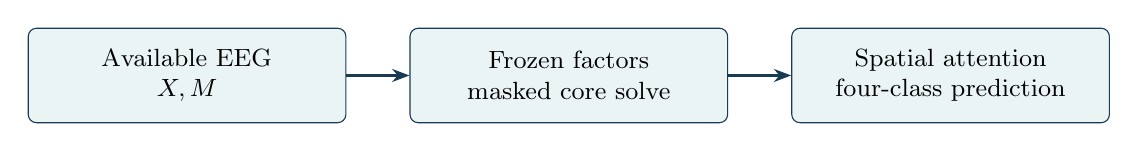
\begin{tikzpicture}
\node[box,text width=38mm] (obs) {Available EEG\\\(X,M\)};
\node[box,text width=38mm,right=8mm of obs] (core) {Frozen factors\\masked core solve};
\node[box,text width=38mm,right=8mm of core] (att) {Spatial attention\\four-class prediction};
\draw[arrow] (obs)--(core);
\draw[arrow] (core)--(att);
\end{tikzpicture}\par
\vspace{14mm}
\textbf{Central question.} Can a shared, low-rank channel--feature model preserve
classification information when known EEG electrodes disappear, compared with
attention receiving the same available features directly?

\textbf{Working hypothesis.} Training-fitted structure may reduce degradation
under electrode loss. It may also discard useful information or hurt full-input
accuracy. The experiment is designed to measure both possibilities.

\vfill
\note{This is an explanation of the supplied code and configuration, not an
experimental-results paper. No accuracy gain has been measured or verified in
this documentation task. The original proposal and current implementation are
explicitly distinguished.}
\vspace{5mm}
\textbf{Reviewed source:} \code{84ae174} (\code{v0.13})\\
\textbf{Review date:} 1 October 2026\\
\textbf{Primary entry points:} \code{run.py}, \code{configs/study.json}\\
\textbf{Editable source:} \code{docs/concept/agfl_concept.tex}
\end{titlepage}
\hypersetup{pageanchor=true}
\pagenumbering{arabic}

\section{Research question and scope}
EEG records voltage signals at named scalp electrodes. The supplied study
classifies four motor-imagery tasks: left hand, right hand, both feet, and tongue.
BCI Competition IV 2a provides nine participants, 22 EEG channels, and recordings
at 250 Hz; three EOG channels are excluded from classifier inputs \cite{bci}.

An electrode can be unavailable throughout a trial or disappear and return
between windows. The classifier receives the availability mask explicitly.
The question concerns robustness to known missing sensors, rather than discovery
of unknown sensor identities or recovery of raw waveforms.

\subsection{Why use a tensor?}
For one trial, collect window-local learned features in
\begin{equation}
 X\in\R^{C\times P\times F},\qquad
 M\in\{0,1\}^{C\times P},\qquad (C,P,F)=(22,4,32).
\end{equation}
Here \(M_{cp}=1\) means electrode \(c\) is observed in window \(p\). Electrode
positions remain fixed when channels disappear. The mask broadcasts over the
feature index \(f\); absence is distinct from a measured numerical zero.

Shared Tucker factors describe channel and feature structure. A new trial's
core is inferred from only its observed entries. Attention then receives a
fixed set of latent spatial tokens. Tensor decomposition provides a structured
model of the feature array \cite{tucker}; arranging features in an array alone
does not provide a reconstruction mechanism.

\subsection{What is implemented?}
\begin{itemize}
\item An EEGNet-derived, channel/window-local encoder shared and frozen across
      all downstream arms \cite{eegnet}.
\item Baseline and Tucker-core representations with MHA and Performer
      \cite{attention,performer}.
\item MHA controls for tensor completion, separable linear compression, and
      training-mean completion.
\item Full and mixed downstream training; evaluation with static and dynamic
      random or spatially grouped channel loss.
\end{itemize}

\note{The current study is participant-specific and within-session. It does not
implement the proposal's subject-disjoint folds, fixed spectral features,
temporal-position tokens, or Nystr\"om attention. Signal Transformer is present
in the library but is outside this study's comparison matrix.}

\textbf{Reader's route.} The following pages explain preprocessing and calibration,
the factor model, exact inference, attention, outage masks, the experiment matrix,
evaluation, and the limits of the implementation.
\source{docs/project_overview.md; configs/study.json; references/proposal_extracted.txt}

\clearpage
\section{Pipeline and separation of fitting from inference}
Each usable trial starts at the cue and contains 1,000 samples per electrode.
Four nonoverlapping 250-sample windows each represent one second. The loader
excludes artifact-marked, boundary-crossing, and unusable/nonfinite trials.

Each window is filtered independently using a fourth-order 2--30 Hz Butterworth
SOS zero-phase filter. This is offline processing. Independent windows prevent
filtering across a hidden interval; the protocol is not causal online inference.

\begin{figure}[h!]
\centering
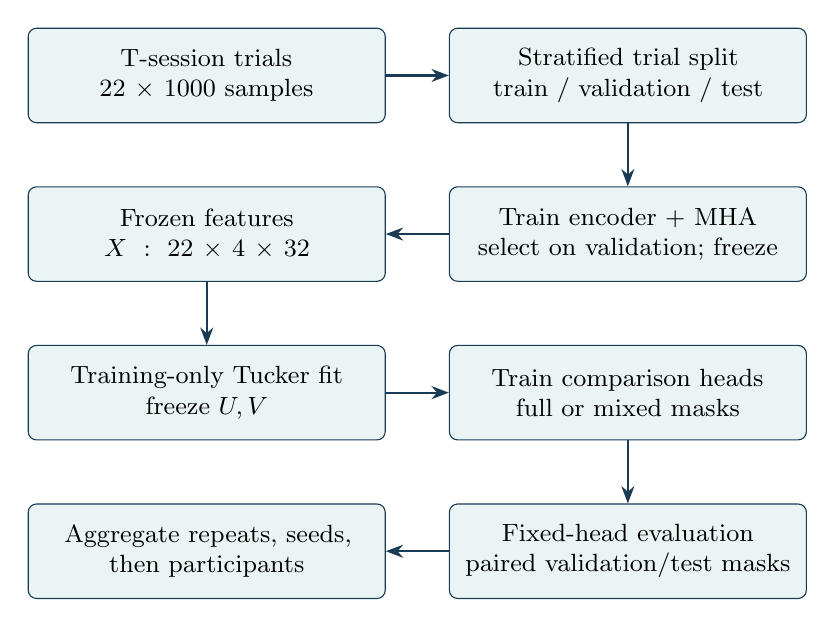
\begin{tikzpicture}[node distance=8mm and 8mm]
\node[box] (data) {T-session trials\\\(22\times1000\) samples};
\node[box,right=of data] (split) {Stratified trial split\\train / validation / test};
\node[box,below=of split] (encoder) {Train encoder + MHA\\select on validation; freeze};
\node[box,left=of encoder] (features) {Frozen features\\\(X:22\times4\times32\)};
\node[box,below=of features] (factor) {Training-only Tucker fit\\freeze \(U,V\)};
\node[box,right=of factor] (heads) {Train comparison heads\\full or mixed masks};
\node[box,below=of heads] (eval) {Fixed-head evaluation\\paired validation/test masks};
\node[box,left=of eval] (report) {Aggregate repeats, seeds,\\then participants};
\draw[arrow] (data)--(split);
\draw[arrow] (split)--(encoder);
\draw[arrow] (encoder)--(features);
\draw[arrow] (features)--(factor);
\draw[arrow] (factor)--(heads);
\draw[arrow] (heads)--(eval);
\draw[arrow] (eval)--(report);
\end{tikzpicture}
\caption{Data flow. Normalization and tensor fitting use training trials only.
Validation selects supervised epochs; test data only score the fixed models.}
\end{figure}

\subsection{Shared feature source}
The encoder applies shared temporal convolution (16 filters, kernel 32), a
grouped \(1\times1\) expansion with depth multiplier 2, and separable temporal
convolution with 32 output filters. Pooling by 8 and 16 leaves one temporal
sample per window, yielding 32 features. It does not convolve across electrodes
or window boundaries and is an adaptation of EEGNet, not standard EEGNet's
full-head spatial convolution.

For each participant/seed, full-input MHA-supervised pretraining selects the
encoder on full-input validation. The pretraining head is discarded; the
encoder is frozen, including BatchNorm statistics and dropout behavior.
Raw channel normalization and subsequent channel-feature standardization use
training statistics only. All arms share the resulting feature cache.

\note{The cache contains full trial features for synthetic outages. This is
consistent with the declared simulation because frozen encoding is local to each
channel/window and hidden features are removed before head or core inference.
It does not simulate permanently absent channels during encoder calibration.}
\source{inm/data.py; inm/model.py::EEGWindowEncoder; inm/study.py::_calibrate}

\clearpage
\section{The shared Tucker-2 model}
Compress the channel and feature modes while leaving the window axis explicit:
\begin{align}
 U&\in\R^{C\times R_C}, & V&\in\R^{F\times R_F}, &
 G&\in\R^{R_C\times P\times R_F},\\
 \widehat X_{cpf}&=\sum_{r=1}^{R_C}\sum_{s=1}^{R_F}U_{cr}G_{rps}V_{fs}, &
 \widehat X_p&=UG_pV^\top. \label{eq:tucker}
\end{align}
The configuration declares \(R_C=R_F=4\). Factors \(U,V\) are shared across
trials; the core \(G\) is specific to each trial and its mask. No factor is
learned along time, and no core solve smooths through future windows.

\begin{figure}[h!]
\centering
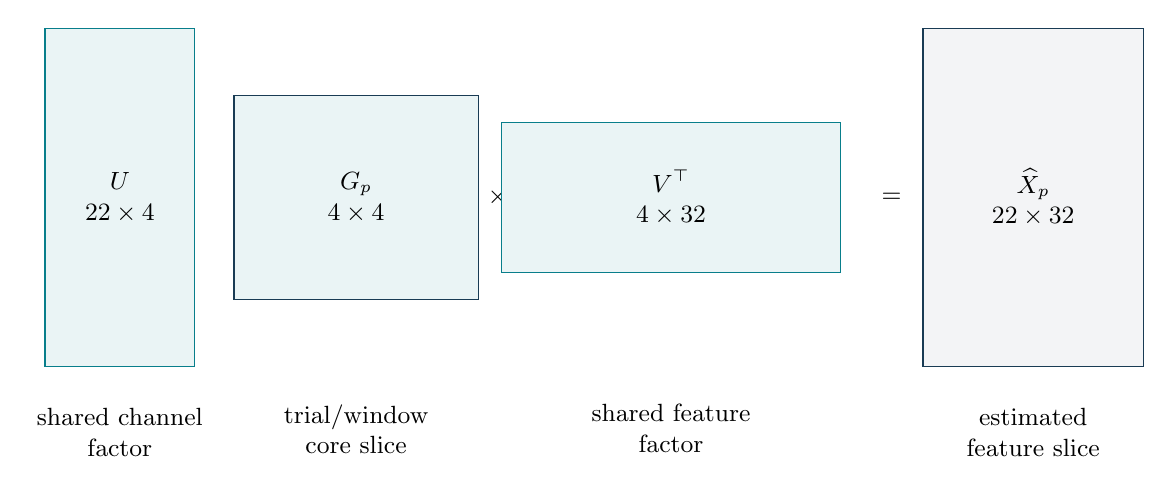
\begin{tikzpicture}[font=\small]
\node[draw=teal,fill=pale,minimum width=19mm,minimum height=43mm,align=center] (u) at (0,0) {\(U\)\\\(22\times4\)};
\node at (1.7,0) {\(\times\)};
\node[draw=navy,fill=pale,minimum width=31mm,minimum height=26mm,align=center] (g) at (3,0) {\(G_p\)\\\(4\times4\)};
\node at (4.8,0) {\(\times\)};
\node[draw=teal,fill=pale,minimum width=43mm,minimum height=19mm,align=center] (v) at (7,0) {\(V^\top\)\\\(4\times32\)};
\node at (9.8,0) {\(=\)};
\node[draw=navy,fill=missing!40,minimum width=28mm,minimum height=43mm,align=center] (x) at (11.6,0) {\(\widehat X_p\)\\\(22\times32\)};
\node[below=4mm of u,align=center] {shared channel\\factor};
\node[below=12mm of g,align=center] {trial/window\\core slice};
\node[below=15.5mm of v,align=center] {shared feature\\factor};
\node[below=4mm of x,align=center] {estimated\\feature slice};
\end{tikzpicture}
\caption{One window of Tucker-2 reconstruction. Four separate core slices
retain the four windows. Boxes are schematic; dimensions are labeled explicitly.}
\end{figure}

\subsection{Compression and its meaning}
The original feature array has \(22\cdot4\cdot32=2{,}816\) scalar entries per
trial. Its core has \(4\cdot4\cdot4=64\) entries, a 44-fold reduction in this
representation count. The two shared factors contain
\(22\cdot4+32\cdot4=216\) scalars, plus fitted-state bookkeeping.

At attention input, the baseline has 22 tokens per window with 32 source
features each; the core has four tokens with four source features each.
Both token adapters project to attention dimension 32. This reduction does not
measure end-to-end memory, trainable parameter savings, or runtime: core inference,
the feature cache, token adapters, and attention implementation also contribute.

\subsection{Factor coordinates are not anatomy}
Columns are projected to unit Euclidean norm, but are not required to be
orthogonal. Components are learned latent coordinates, not named brain regions
or anatomical connectivity. Factor/core parameterizations admit ambiguities;
freezing the shared factors keeps the coordinates consistent across trial inference.

\note{Low-rank reconstruction may suppress noise, but it may also suppress class
information. A fixed latent shape and a low reconstruction error are insufficient
evidence of improved classification.}
\source{inm/tensor_attention.py::Tucker2; configs/study.json::tensor}

\clearpage
\section{Exact core inference from observed features}
For window \(p\), let \(O_p=\{c:M_{cp}=1\}\), \(n_p=|O_p|\), and
\(D_p=n_pF\), the number of observed scalar features. Holding factors fixed,
infer the core by normalized ridge regression:
\begin{equation}
 G_p^*=\arg\min_{G\in\R^{R_C\times R_F}}
 \ell_p(G),\qquad
 \ell_p(G)=\frac{\|X_{O_p,p,:}-U_{O_p,:}GV^\top\|_F^2}{D_p}
             +\lambda\|G\|_F^2. \label{eq:ridge}
\end{equation}
The declared ridge is \(\lambda=10^{-3}\). Hidden channels do not occur in the
data term; inference uses neither labels nor hidden reference features.

\subsection{Normal equations}
Differentiating Equation~\eqref{eq:ridge} and multiplying by \(D_p/2\) gives
\begin{equation}
 A_pG_pB+D_p\lambda G_p=T_p,
 \quad A_p=U_{O_p,:}^\top U_{O_p,:},\quad
 B=V^\top V,\quad T_p=U_{O_p,:}^\top X_{O_p,p,:}V. \label{eq:normal}
\end{equation}
The observation normalization matters: the ridge coefficient in the normal
equation is \(D_p\lambda\), rather than \(\lambda\) alone.

Let \(A_p=Q_p\operatorname{diag}(a_p)Q_p^\top\) and
\(B=S\operatorname{diag}(b)S^\top\) be symmetric eigendecompositions. With
\(H_p=Q_p^\top T_pS\), Equation~\eqref{eq:normal} reduces to entrywise division:
\begin{equation}
 (\widetilde G_p)_{ij}=\frac{(H_p)_{ij}}{(a_p)_i b_j+D_p\lambda},
 \qquad G_p^*=Q_p\widetilde G_pS^\top. \label{eq:eigen}
\end{equation}
Gram matrices are symmetrized, roundoff-negative eigenvalues clipped to zero,
and solves computed in float64. With \(n_p\geq1\) and positive ridge, every
denominator is positive, so the conditional core is unique even with deficient
observed-channel rank. Statistical recovery is a separate question.

\subsection{Numerical and missingness safeguards}
Select observed entries before any arithmetic:
\[
 X^{\rm safe}_{cpf}=\begin{cases}X_{cpf},&M_{cp}=1,\\0,&M_{cp}=0.\end{cases}
\]
The implementation uses \code{torch.where}. Multiplication is unsuitable for
unknown placeholders because \(0\cdot\mathrm{NaN}=\mathrm{NaN}\).
Observed features must be finite and every trial/window must retain a channel.
The low-level solver accepts any positive observed count; the declared study
uses at least six. Core inference is detached and does not update the factors.

\subsection{Learning the factors}
On training trials only, minimize
\[
 \frac{1}{N_{\rm train}P}\sum_{n\in D_{\rm train}}\sum_{p=1}^{P}
 \ell_p(G_{np};U,V,X_n,M_n),\quad
 \|U_{:r}\|_2=\|V_{:s}\|_2=1.
\]
Each minibatch alternates exact core solves and Adam factor updates with cores
held fixed, followed by column normalization. The study uses 30 epochs on full
training features. This nonconvex projected alternating fit has no stated global
optimality guarantee. Fitted factors become buffers outside classifier optimizers.
\source{inm/tensor_attention.py::_solve, _objective, fit, encode}

\clearpage
\section{Representations, spatial attention, and readout}
The tensor route uses \(G\) directly. Its separate completion control fills
missing features while preserving observed values exactly:
\begin{equation}
 X^{\rm comp}_{cpf}=\begin{cases}
 X_{cpf},&M_{cp}=1,\\(UG_pV^\top)_{cf},&M_{cp}=0.
 \end{cases} \label{eq:completion}
\end{equation}
Completion estimates features, not raw EEG. Its original mask remains an input.
The linear control computes \(G^{\rm lin}_p=W_C X^{\rm safe}_pW_F^\top\), with
trainable separable maps and the same core shape. Mean completion inserts the
training channel-feature mean, which is close to zero after standardization.

\subsection{Tokens and availability information}
For window \(p\), let \(t_{jp}\) denote the represented feature vector and
\(m_p=M_{:p}\). Tokens are constructed as
\begin{equation}
 z_{jp}=W_{\rm in}t_{jp}+b_{\rm in}+a_j
             +w_{\rm status}s_{jp}+W_Mm_p.
\end{equation}
Here \(a_j\) is a learned electrode or component identity. For electrode tokens,
\(s_{jp}=M_{jp}\); for latent tokens, \(s_{jp}=n_p/C\). Baseline missing tokens
replace the projected feature term with a learned placeholder. All arms receive
the full observed-channel mask; there is no temporal position term.

\subsection{Two attention families}
Each window is processed independently by a residual attention/FFN block.
For one MHA head, with \(d_h=32/4=8\), standard attention is \cite{attention}
\begin{equation}
 Q=ZW_Q,\quad K=ZW_K,\quad L=ZW_L,\qquad
 A(Z)=\operatorname{softmax}\!\left(\frac{QK^\top}{\sqrt{d_h}}\right)L.
\end{equation}
The value symbol \(L\) avoids confusing attention values with tensor factor \(V\).
Performer approximates the softmax kernel through a positive random-feature map
\(\phi\), allowing the reassociation \cite{performer}
\begin{equation}
 A_i(Z)\approx
 \frac{\phi(q_i)^\top\bigl(\phi(K)^\top L\bigr)}
      {\phi(q_i)^\top\sum_j\phi(k_j)}.
\end{equation}
The implementation uses 64 fixed orthogonal random features per head, stabilized
exponentials, and a denominator floor. Neither attention module receives an exact
key-padding mask; missingness enters through token construction.

\subsection{Pooling and prediction}
Let \(h_{jp}\) be the final normalized tokens and \(w_{jp}\) the pooling weights:
\begin{equation}
 h_p=\frac{\sum_jw_{jp}h_{jp}}{\sum_jw_{jp}},\qquad
 \bar h=\frac1P\sum_p h_p,\qquad
 \pi=\operatorname{softmax}(W_o\bar h+b_o).
\end{equation}
Baseline pooling counts observed electrodes only, though missing placeholders
can still participate in attention. Completion pools all electrode tokens;
core routes pool all latent tokens. No declared window is completely absent.
Training uses cross-entropy and AdamW. Window averaging implies invariance to a
joint permutation of feature and mask windows at evaluation.
\source{inm/model.py::FeatureClassifier; agfl/attention/mha/layer.py; agfl/attention/performer/layer.py}

\clearpage
\section{Availability protocol: static and dynamic loss}
Retain \(k\in\{22,16,11,6\}\) electrodes per window. Missing percentages are
\(100(22-k)/22\), giving 0\%, 27.27\%, 50\%, and 72.73\%. Six electrodes are
the supplied integer approximation to roughly three-quarters channel loss.

\begin{center}
\begin{tabularx}{\linewidth}{lY}
\toprule
Pattern & How missing channels are chosen \\
\midrule
Random static & A random subset is kept for every window of a trial. \\
Spatial static & The nearest \(22-k\) electrodes to a sampled center are removed
on fixed schematic scalp coordinates. \\
Dynamic random & Distinct random subsets follow an A--B--A schedule. \\
Dynamic spatial & Distinct spatial-loss subsets follow the same schedule. \\
\bottomrule
\end{tabularx}
\end{center}

\begin{figure}[h!]
\centering
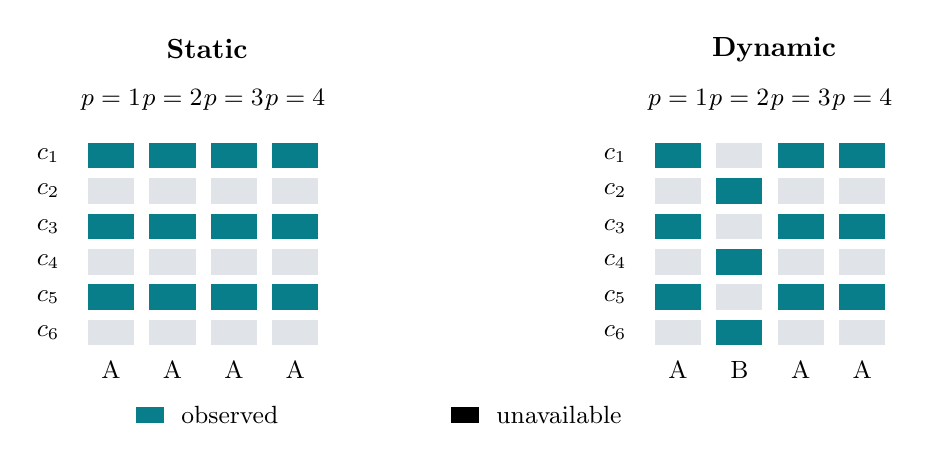
\begin{tikzpicture}[font=\small]
\foreach \grid/\origin/\labeltext in {0/0/Static,1/7.2/Dynamic}{
  \node[font=\bfseries] at (\origin+1.9,4.4) {\labeltext};
  \foreach \p in {1,...,4}{\node at (\origin+\p*.78-.1,3.75) {\(p=\p\)};}
  \foreach \c in {1,...,6}{
    \node[anchor=east] at (\origin+.15,3.5-\c*.45) {\(c_{\c}\)};
    \foreach \p in {1,...,4}{
      \pgfmathtruncatemacro{\keep}{mod(\c,2)}
      \ifnum\grid=1
        \ifnum\p=2\pgfmathtruncatemacro{\keep}{1-\keep}\fi
      \fi
      \ifnum\keep=1\def\cellcolor{teal}\else\def\cellcolor{missing}\fi
      \filldraw[fill=\cellcolor,draw=white] (\origin+\p*.78-.4,3.5-\c*.45-.17)
        rectangle ++(.6,.34);
    }
  }
  \foreach \p/\txt in {1/A,2/A,3/A,4/A}{
    \ifnum\grid=1\ifnum\p=2\def\txt{B}\fi\fi
    \node at (\origin+\p*.78-.1,.32) {\txt};
  }
}
\fill[teal] (1,-.35) rectangle ++(.35,.2);
\node[anchor=west] at (1.45,-.25) {observed};
\fill[missing] (5,-.35) rectangle ++(.35,.2);
\node[anchor=west] at (5.45,-.25) {unavailable};
\end{tikzpicture}
\caption{Illustrative six-channel universe retaining three channels, rather than
an actual BCI mask. The same observed count is kept in every window. For the
study's four windows, the dynamic schedule is A, B, A, A.}
\end{figure}

The general dynamic rule uses B on
\([\lfloor P/3\rfloor,\lfloor2P/3\rfloor)\) in zero-based window indices and
A elsewhere. Reappearing channels retain their original identities.
Schematic spatial coordinates define clustered loss, not measured anatomy.

\subsection{Training and evaluation masks}
Full training observes all 22 channels. Mixed training draws 22, 16, or 6
uniformly per trial/epoch; degraded trials choose random static or random dynamic
loss uniformly. Eleven-channel inputs and spatial patterns are evaluation-only.

SHA256-based keys use participant, seed, partition, trial identity, condition,
and repeat or training epoch, excluding attention and representation identity.
Nonfull channel subsets are canonically assigned to train, validation, or test
by hashing their original electrode bitset modulo three. Rejection sampling
enforces that assignment across patterns; the full subset is the shared exception.
Thus compared arms receive identical masks without reusing nonfull subsets
across data partitions.
\source{inm/availability.py::make_mask_bank, training_mask_bank, subset_partition}

\clearpage
\section{The declared experiment}
For each participant A01--A09 and seed 0, 1, or 2, stratify that participant's
T-session trials into approximately 60\% training, 20\% validation, and 20\% test.
Fractions are rounded within class. No participants are pooled during training.

\begin{center}
\begin{tabularx}{\linewidth}{Yccc}
\toprule
Representation & MHA & Performer & Regimes \\
\midrule
Baseline & yes & yes & full, mixed \\
Tucker core & yes & yes & full, mixed \\
Tensor completion & yes & --- & full, mixed \\
Separable linear core & yes & --- & full, mixed \\
Training-mean completion & yes & --- & full, mixed \\
\bottomrule
\end{tabularx}
\end{center}
There are \((2\cdot2+3)\cdot2=14\) heads per participant/seed and
\(9\cdot3=27\) tasks, totaling \(378\) downstream classifier fits. In addition,
there are 27 shared encoder fits and 27 Tucker calibrations. Each calibrated
encoder/factor pair is reused by all 14 downstream heads in its task.

\subsection{Budgets and selection}
\begin{center}
\begin{tabularx}{\linewidth}{lY}
\toprule
Setting & Supplied value \\
\midrule
Supervised training & Cross-entropy, AdamW, batch size 32, at most 250 epochs \\
Learning rate & Target \(10^{-3}\); 10-epoch warmup, then cosine schedule \\
Regularization & Weight decay \(10^{-4}\), gradient clipping norm 1 \\
Early stopping & At least 75 epochs; patience 50 \\
Encoder dropout & 0.5 \\
Head & Dimension 32, four heads, one attention/FFN block, dropout 0.1 \\
Factor fitting & 30 epochs; learning rate 0.01; batch size 64; ridge 0.001 \\
Mask repeats & One full-input condition; five repeats per degraded condition \\
\bottomrule
\end{tabularx}
\end{center}
The best full-input validation balanced accuracy selects the epoch;
unweighted validation log loss breaks ties. Both downstream availability regimes
use full-input validation for selection. There is no test-based rank search or
arm-specific tuning in the supplied configuration.

\subsection{Evaluation coverage and controls}
One full condition and four patterns at each of three degraded counts give 13
scenarios. Repeats produce \(1+3\cdot4\cdot5=61\) evaluations per partition per
head, or 122 across validation and test. Heads are fixed; individual outage
conditions do not trigger retraining.

Completion tests imputation in electrode space. Linear-core control tests
supervised separable compression. Mean completion provides simple imputation.
These controls differ in objectives, capacity, token count, and pooling; equal
latent shape does not imply equal trainable parameter counts.
\source{configs/study.json; inm/protocol.py::arms, tasks; inm/training.py::fit}

\clearpage
\section{Outcomes and paired statistical comparisons}
For four classes, balanced accuracy averages class recalls:
\begin{equation}
 \operatorname{BA}=\frac14\sum_{a=1}^4\frac{TP_a}{TP_a+FN_a}.
\end{equation}
Macro-F1 averages per-class F1,
\(\operatorname{F1}_{\rm macro}=\frac14\sum_a
2TP_a/(2TP_a+FP_a+FN_a)\), with metric edge cases handled by the implementation.
Balanced accuracy is primary; accuracy, macro-F1, and reconstruction are secondary.

\subsection{Aggregation and gains}
Let \(b^{(m)}_{sekrg}\) be balanced accuracy for method \(m\), participant \(s\),
seed \(e\), retained count \(k\), mask repeat \(r\), and loss pattern \(g\),
for a fixed attention family and training regime. First average mask repeats,
then three seeds, then nine participant means:
\begin{equation}
 \bar b^{(m)}_{skg}=\frac13\sum_{e=1}^3
   \frac1{R_{kg}}\sum_{r=1}^{R_{kg}}b^{(m)}_{sekrg},\qquad
 S^{(m)}_{kg}=\frac19\sum_{s=1}^9\bar b^{(m)}_{skg}.
\end{equation}
Participants have equal weight. Neither masks nor seeds are independent participants.
For matched Tucker-core and baseline heads, define percentage-point gains
\begin{equation}
 \Delta_{skg}=100\bigl(\bar b^{(T)}_{skg}-\bar b^{(B)}_{skg}\bigr),\qquad
 \Delta_{kg}=\frac19\sum_s\Delta_{skg}.
\end{equation}
Positive gain favors the tensor route. Positive degradation means a drop from
the method's full-input score:
\(D^{(m)}_{kg}=100(S^{(m)}_{22}-S^{(m)}_{kg})\).
For each loss pattern, the robustness summary is
\begin{equation}
 \mathcal R^{(m)}_g=\frac14\left(S^{(m)}_{22}+S^{(m)}_{16,g}
                    +S^{(m)}_{11,g}+S^{(m)}_{6,g}\right).
\end{equation}
It is an equal-weight four-condition average, not a continuous-curve area.

\subsection{Uncertainty and incomplete results}
Resample the nine participant-level paired differences with replacement 2,000
times. The 2.5th and 97.5th percentiles of resampled means form pointwise 95\%
bootstrap intervals. Subject standard deviation is reported separately.
These intervals are exploratory and not multiple-comparison corrected.
Paired mask hashes must agree; incompatible pairs are excluded visibly.
All-participant means remain blank until every required fit is complete.

\subsection{Hidden-feature reconstruction}
Only after inference, evaluate artificial hidden entries against reference features:
\begin{equation}
 \operatorname{NRMSE}_{\rm hid}=
 \sqrt{\frac{\sum_{c,p,f:M_{cp}=0}(\widehat X_{cpf}-X_{cpf})^2}
                 {\sum_{c,p,f:M_{cp}=0}X_{cpf}^2}}.
\end{equation}
The study pools sums over the evaluated partition in standardized feature space.
No hidden entries or zero reference energy yields an undefined/blank value.
This exact implementation has no additive epsilon in the denominator.
Reconstruction scores neither fit factors nor select heads.
\source{inm/training.py::metrics; inm/reporting.py; inm/study.py::_reconstruction_scores}

\clearpage
\section{Proposal fidelity, limitations, and collaboration priorities}
\begin{center}
\small
\begin{tabularx}{\linewidth}{YY}
\toprule
Original proposal & Supplied implementation \\
\midrule
Fixed channel-wise time--frequency features & Frozen supervised EEGNet-derived window features \\
Three subject-disjoint folds & Nine individually trained participants; within-T-session trial splits \\
Component--window tokens with time positions & Spatial attention separately per window; order-invariant averaging \\
MHA, Nystr\"om-style, Performer-style & MHA and Performer; no Nystr\"om implementation \\
Small validation-only rank search & Fixed ranks \(R_C=R_F=4\), without an executed rank search \\
Tensor core and completion controls & Both, plus separable linear and training-mean controls \\
Varying availability and held-out patterns & Full/mixed head training; held-out 11-channel and spatial losses \\
\bottomrule
\end{tabularx}
\end{center}

\subsection{What the study can establish}
If executed correctly, the study can compare frozen-representation behavior
under declared channel losses and quantify full-input costs, per-participant
variation, and paired core-versus-baseline changes. It can examine whether
compression, completion, or mixed-mask training explains robustness.

It cannot establish unseen-participant generalization, the official train-on-T /
test-on-E benchmark, causal online performance, anatomical connectivity, or a
gain for standard end-to-end EEGNet. Full-channel calibration is assumed.
MHA-based feature pretraining may favor MHA. Severe spatial loss can remove
information that no factor model can reconstruct. The short spatial sequences
do not themselves support a Performer speed claim.

\subsection{Readiness at the reviewed workstation}
The dependency-light task planner runs and confirms 27 tasks and 378 heads.
Python 3.13.13 and the LaTeX toolchain are available. PyTorch, NumPy, SciPy,
scikit-learn, and MNE are absent; the default \code{../ml} data directory and saved
results are absent. Consequently, numerical inference, training, CUDA behavior,
and performance are unverified here. No checked-in tests or Slurm launcher were
found. Dataset helpers are present; a broad ignore rule hides them from ordinary
file searches, so use the tracked Git inventory.

\subsection{Suggested next steps with the supervisor}
\begin{enumerate}
\item Agree on the intended scientific protocol: this participant-specific study,
      the original subject-disjoint proposal, or a separate cross-session design.
\item Provision the scientific environment and official GDF recordings on the
      experiment machine; inspect a single participant/seed task first.
\item Add numerical checks for the ridge solve, hidden-NaN isolation, observed
      completion values, mask separation, and incomplete-pair reporting.
\item Preserve source/configuration/data identities, report unfavorable outcomes,
      and interpret controls before attributing improvements to tensor structure.
\end{enumerate}
\source{references/proposal_extracted.txt; docs/investigation.md; docs/experiment.md}

\clearpage
\section{Reproducing the document and navigating the repository}
\textbf{Orientation files.} \code{docs/README.md} indexes the existing technical
notes. \code{docs/onboarding.md} provides a guided collaborator workflow;
\code{docs/investigation.md} records dated evidence and readiness.
Root \code{AGENTS.md} supplies future assistant context and research invariants.

\textbf{Code ownership.} \code{inm/} owns the experiment, masking, representations,
training orchestration, reporting, and plots. \code{agfl/} owns EEG model,
attention, data/split, optimization, and reproducibility helpers.
\code{references/} contains the proposal as PDF, DOCX, and extracted text.

\textbf{Useful commands from the repository root:}
\begin{lstlisting}
# Dependency-light plan; no training
python run.py --config configs/study.json --plan

# On a provisioned CUDA/data machine: A01, seed 0, all 14 heads
python run.py --config configs/study.json --task-index 0

# After saved results exist
python run.py --config configs/study.json --summarize-only
python run.py --config configs/study.json --summarize-only --plots

# Rebuild this PDF without Python or external images
make -C docs/concept
\end{lstlisting}

The report entry point is \code{results/inm-v2/report/summary.md}. Keep
\code{artifacts/} for calibration, splits, histories, and provenance. Selected
head weights are evaluated in memory and are not saved as standalone checkpoints.
Changed code/packages/configuration require a new compatible study output
directory; do not mix incompatible runs.

\begingroup
\small
\begin{thebibliography}{9}
\bibitem{bci} C. Brunner et al. \emph{BCI Competition 2008: Graz data set A
(BCI Competition IV, data set 2a)}. Official dataset description.
\href{https://www.bbci.de/competition/iv/desc_2a.pdf}{bbci.de/competition/iv/desc\_2a.pdf}.
\bibitem{tucker} T. G. Kolda and B. W. Bader. \emph{Tensor Decompositions and
Applications}. SIAM Review 51(3), 455--500, 2009.
\href{https://www.kolda.net/publication/koba09/}{Author's publication page};
\href{https://doi.org/10.1137/07070111X}{doi:10.1137/07070111X}.
\bibitem{eegnet} V. J. Lawhern et al. \emph{EEGNet: A Compact Convolutional
Network for EEG-based Brain--Computer Interfaces}. Journal of Neural Engineering,
2018. \href{https://arxiv.org/abs/1611.08024}{arXiv:1611.08024}.
\bibitem{attention} A. Vaswani et al. \emph{Attention Is All You Need}. NeurIPS,
2017. \href{https://arxiv.org/abs/1706.03762}{arXiv:1706.03762}.
\bibitem{performer} K. Choromanski et al. \emph{Rethinking Attention with
Performers}. ICLR, 2021. \href{https://arxiv.org/abs/2009.14794}{arXiv:2009.14794}.
\bibitem{proposal} \emph{Tensor-Structured Attention for Classification under
Variable Signal Availability}. Repository proposal in \code{references/};
author/date unspecified in the extracted text.
\bibitem{repo} AGFL-inm repository, reviewed revision \code{84ae174},
\code{configs/study.json}, \code{inm/}, \code{agfl/}, and \code{docs/}.
Reviewed 1 October 2026. Equations and settings describe this source snapshot.
\end{thebibliography}
\endgroup
\end{document}
